% !TeX program = pdfLaTeX
\documentclass[12pt]{article}
\usepackage{amsmath}
\usepackage{amsthm}
\usepackage{graphicx,psfrag,epsf}
\usepackage{enumerate}
\usepackage{natbib}
\usepackage{booktabs}
\usepackage{longtable}
\usepackage{array}
\usepackage{multirow}
\usepackage[table]{xcolor}
\usepackage{wrapfig}
\usepackage{float}
\usepackage{colortbl}
\usepackage{hyperref}
\usepackage{pdflscape}
\usepackage{tabu}
\usepackage{threeparttable}

\usepackage{url} % not crucial - just used below for the URL

%\pdfminorversion=4
% NOTE: To produce blinded version, replace "0" with "1" below.
\newcommand{\blind}{0}

% DON'T change margins - should be 1 inch all around.
\addtolength{\oddsidemargin}{-.5in}%
\addtolength{\evensidemargin}{-.5in}%
\addtolength{\textwidth}{1in}%
\addtolength{\textheight}{1.3in}%
\addtolength{\topmargin}{-.8in}%

\newenvironment{definition}[1]% environment name 
{% begin code 
  \par\vspace{.75\baselineskip}\noindent 
  \textbf{Definition (#1)}\begin{itshape}% 
  \par\vspace{.5\baselineskip}\noindent\ignorespaces 
}% 
{% end code 
  \end{itshape}\ignorespacesafterend 
}

\providecommand{\tightlist}{%
  \setlength{\itemsep}{0pt}\setlength{\parskip}{0pt}}

\begin{document}

\def\spacingset#1{\renewcommand{\baselinestretch}%
{#1}\small\normalsize} \spacingset{1}


%%%%%%%%%%%%%%%%%%%%%%%%%%%%%%%%%%%%%%%%%%%%%%%%%%%%%%%%%%%%%%%%%%%%%%%%%%%%%%

\if0\blind
{
  \title{\bf Adaption of the Chumbley Score to matching of bullet striation marks}

  \author{
        Ganesh Krishnan \thanks{The authors gratefully acknowledge \ldots{}} \\
    Department of Statistics, Iowa State University\\
     and \\     Heike Hofmann \\
    Department of Statistics and CSAFE, Iowa State University\\
      }
  \maketitle
} \fi

\if1\blind
{
  \bigskip
  \bigskip
  \bigskip
  \begin{center}
    {\LARGE\bf Adaption of the Chumbley Score to matching of bullet striation marks}
  \end{center}
  \medskip
} \fi

\bigskip
\begin{abstract}

\end{abstract}

\noindent%
{\it Keywords:} 3 to 6 keywords, that do not appear in the title
\vfill

\newpage
\spacingset{1.45} % DON'T change the spacing!

\newcommand{\hh}[1]{{\textcolor{orange}{#1}}}
\newcommand{\gk}[1]{{\textcolor{green}{#1}}}
\newcommand{\cited}[1]{{\textcolor{red}{#1}}}

\tableofcontents
\newpage

\section{Introduction and Background}\label{introduction-and-background}

\subsection{Motivation}\label{motivation}

Same source analyses are a major part of an Forensic Toolmark Examiner's
job. In current practice examiners make these comparisons visually under
a comparison microscope and come to one of the following four
conclusions: identification, inconclusive, elimination or unsuitable for
examination \citet{afte-website-2}. These conclusions are made on the
basis of ``unique surface contours'' of the two toolmarks being in
``sufficient agreement'' \citep{afte-toolmarks1998}. AFTE describes the
term ``sufficient agreement'' as the possibility of another tool
producing the markings under comparison, as practically impossible
\citep{afte-toolmarks1998} \citep{afte-website}.
\%\gk{Although, they go on to concede that the interpretation of the identification depends on the examiner and is  therefore subjective in nature.}
This subjectivity in the assessment as well as the lack of error rates
are the main points of criticisms in the toolmark examination first
raised by the National Research Council in 2009 \citep{NAS:2009} and
later emphasized further by the President's Council of Advisors on
Science and Technology \citep{pcast2016}.

Technological advances, such as profilometers and confocal microscopy
allow to measure 3D surfaces \citep{vorburger2016} in a digitized form.
This forms the basis of statistical analysis of toolmarks. A statistical
approach based on data removes both subjectivity from the assessment and
allows a quantification of error rates for both false positive and false
negative identifications.

Various toolmarks have been studied in the literature: screwdriver marks
digitized using a profilometer have been analyzed in
\citet{manytoolmarks1} and \citet{chumbley}; \citet{manytoolmarks2} have
investigated 3D marks from screwdriver, tongue and groove pliers
captured using a confocal microscope; digitized marks from slip-joint
pliers generated by a surface profilometer have been investigated by
\citet{afte-chumbley}.

\citet{manytoolmarks2} define a relative distance metric and use it as
similarity measure between two toolmarks. \citet{manytoolmarks1} extract
many small segments in the markings of two toolmarks and compare
similiarity using a maximum pearson correlation coefficient. The
Chumbley scoring method, first introduced by \citet{chumbley}, uses a
similar but more extensive framework based on a Mann-Whitney U test of
the resulting correlation coefficients. This approach was later improved
by Hadler and Morris \citep{hadler}.
\hh{XXX describe the improvement in half a sentence XXX} In this paper,
we are investigating the applicability of the Chumbley scoring method by
\citet{hadler} to assess striation marks on bullet lands for same-source
identification.

Striation marks on bullets are made by impurities in the barrel. As the
bullet travels through the barrel, these imperfections leave
``scratches'' on the bullet surface. Typically, only striation marks in
the land engraved areas (LEAs) are considered \citet{afte-article1992}.
Bullet lands are depressed areas between the grooves made by the rifling
action of the barrel. Compared to toolmarks made by screwdrivers
striation marks on bullets are typically much smaller, both in length
and in width. Bullets also have a curved cross-sectional topography
\hh{sketch?}.

Bullet matching methods depend on the attribute being used for making
comparisons. For single feature based matching \citet{chu2013} used an
automatic method for counting consequtive matching striae (CMS). They
reported zero false positive rate but do not discuss about the false
negative rates for land to land matches. \citet{ma2004} and
\citet{vorburger2011} discuss about CCF (cross-correlation function) and
its discriminating power and application but do not talk about matches
and non-matches. \citet{aoas} use multiple attributes like CCF, CMS, D
(distance measure) etc in a random forrest based method and compare
every land against every other land of the Hamby dataset \citet{hamby}.
They report an out-of-bag error rate with false positive error rate of
0.0001 and false negative error rate of 0.2267 for 100 trees. For 300
trees they report correct prediction of all matches and non-matches.

The Chumbley score provides us with another approach in the same-source
assessment of bullet striation marks. \citet{chumbley}, in their paper,
compare two toolmarks with the intention of determining if it comes from
the same tool. The data for their study was obtained from 50
sequentially manufactured screwdriver tips.\citet{chumbley} reported
error rates for marking made by the tips at differnt angles. For a 30
degree they showed false negative error rate to be 0.023 and false
positive error rate be 0.09. For other angles the error rates remain the
same for false negatives and 0.01 for false positives. The improvement
proposed by \citet{hadler} on the other hand, did not consider effect of
angles and gave 0.06 false negative error rate and 0 false poisitive
error rate for markings made at the same angle.

\gk{\citep{afte-website} quotes sufficient agreement as "agreement of individual characteristics is of a quantity and quality that the likelihood another tool could have made the mark is so remote as to be considered a practical impossibility"}
\gk{could not find the pdf for AFTE theory of identification as it relates to toolmarks pdf. I believe it is not available for free. But from the AFTE Journal the abstract was available which mentions the term " sufficient agreement" as quoted above. Currently the website seems like the most reliable way of quoting AFTE, i have checked other sources in both occasions where the website has been quoated above, like an FBI paper available at the FBI website \citet{fbi-paper} and some non published but available pdf files in the AFTE website that have used these lines and quoted the AFTE journal. But since I cannot verify it in the Journal I have quoated the website.}
\gk{faden et al have not cited any paper that discusses the algorithm, i assume it was developed for the paper, the discussion of which is not as extensive as chumbley's. Its a variation of the chumbley method but from my understanding it is just the optimization step. and this paper came out much before the chumbley score.}

\hh{XXX first sentence: Same source analyses are a major part of an Forensic Toolmark examiners job. XXX second sentence: describe standard practice: In current practice firearm examiners  make these comparisons visually under a comparison microscope and report XXX what is being reported: AFTE. XXX find: AFTE theory of identification as it relates to toolmarks  }
\hh{One of the main criticisms in this toolmark examination first raised by the National Research Council in 2009 [@NAS:2009] and later emphasized further by the President's Council of Advisors on Science and Technology [@pcast2016] are the amount of subjectivity in the assessment and the lack of error rates. }
\hh{XXX we have digitized images, e.g. profilometers or Confocal microscopy allow us to measure the surface [@vorburger2016]}

\hh{Using a statistical approach removes both subjectivity from the assessment and allows us to provide error rates for both false positive and false negative identifications. }
\hh{Multiple toolmarks have been studied in the literature:  \citep{manytoolmarks1, manytoolmarks2, chumbley} have studied screwdriver marks digitized using a profilometer,  \citep{manytoolmarks2} investigate groove pliers XXX data? XXX  to slip-joint pliers \citep{afte-chumbley} XXX. In all of these cases, the statistical test used, is a variation of the Chumbley scoring method, first introduced by XXX and later improved by XXX. }

\hh{XXX In this paper, we are investigating the applicability of the Chumbley scoring method by @hadler to assessing striation marks on bullets for same-source identification. }

\hh{Striation marks on bullets are made by impurities in the barrel. As the bullet travels through the barrel, these imperfections leave "scratches" on the bullet surface. Typically, only striation marks in the land engraved areas (LEAs) are considered (XXX citation) [@afte-article1992]. XXX explain lands and grooves XXX. Compared to toolmarks made by screwdrivers striation marks on bullets are typically much smaller, both in length and in width. Bullets also have a curved cross-sectional topography. 
}

\hh{XXX How are bullets matched now? \citet{chu2013}: CMS, automatically - error rate?, using ccf XXX Vorburger paper XXX  and \citet{aoas}: multiple features, error rates }

\hh{The Chumbley score  provides us with another approach in the same-source assessment of bullet striation marks. }

\hh{end of intro: remaining paper is structured as follows: introduce to the data we get from confocal microscopy, introduce to profiles and signatures.
Introduce to chumbley score method, apply chumbley and discuss results ....
}

\subsection{Scans for land engraved
areas}\label{scans-for-land-engraved-areas}

\begin{itemize}
\tightlist
\item
  scans available: NIST database (citation), Hamby 44 and Hamby 252
  (Hamby citation)
\item
  move figure up
\item
  discuss cross section, profiles and signatures
\end{itemize}

Compairing pairs of toolmarks with the intention of matching it to a
tool has been studied many times in the past. Extensive examples can be
found in literature for tools and toolmark research ranging from
screwdrivers \citep{manytoolmarks1, manytoolmarks2, chumbley} to groove
pliers \citep{manytoolmarks2} to slip-joint pliers \citep{afte-chumbley}
and many more. In comparison to this, same source matching of bullets to
firearms has not been examined as prominently as that of toolmarks. Even
less information is available on validity of methods and error rates
associated with firearms examination. The National Academy of Sciences
in its report in 2009 \citep{NAS:2009} discussed the need for
determining error rates in methods proposed for firearms examination. As
seen in the case of most forensic applications, the first step for same
source matching and error rate determination involves identification of
unique features that are characteristic of the object at hand. For the
case of bullets and firearms, striation marks on the surface of the
bullet are considered to be such markings that can be used in methods
for same source matching. These marks are often a product of rifling and
impurities and defects due to manufacturing in the barrel of the gun,
which leads to engravings on the bullet surface
\citep{afte-article1992}. In current practice, firearm examiners
invariably make visual comparisons of bullet striae and use visual
assesment tools to dignify bullets as being matches and non-matches. One
way of accomplishing anykind of comparison between bullets is to do a
comparison between surface marking of two or more bullet lands. Bullet
Lands are considered to be areas between grooves made by the rifling
action of the barrel and the markings on them are considered to be
unique. The land engraved markings or sometimes termed as Bullet
profiles \citep{aoas,ma2004} are striation marks made on Bullet lands
and often used for these land to land comparisons. Bullet Signatures is
another word used in literature as seen in the work of \citet{chu2013}
and \citet{aoas}. In our context bullet signatures refer to a processed
version of the raw land engraved markings or profiles. The generation of
bullet signatures involves first extraction of a bullet profile by
taking the cross-sectional of the surface at a given height and then
using loess fits to model the structure. The residuals of this fit are
called signatures, which are considered to be noise free and a good
reflection of the class charecteristics and unique features of a bullet.
A more detailed version of the extraction technique of signatures is
discussed by \citet{aoas}, where comprehensive details about the height
at which profile is to be selected, removing curvature, smoothing,
identifying groove locations are explained. Figure \ref{fig:rgl} shows
us how the extracted signature from a bullet land lines up with the
image of the land from which it was extracted. We can see also see in
the figure how the depth and relative position of the striation markings
seen in the image are interpreted as the signature.

As mentioned earlier, subject bias and error rate determination have
been a long standing issue in firearm examination \citep{NAS:2009}. This
issue of removing subjectivity and making firearm analysis objective was
also raised in the \citet{pcast2016} report. For an objective analysis,
scientific principle testability and error rate determination are
considered to be defining aspects. Identification of the uncertainities
associated with a method of comparison and coming up with a systemized
method of quantification, is therefore important. Associating
mathematical probabilites in a systematic manner to these methods are
one such way of quantification. In a previous study conducted by
\citet{aoas} a machine learning based algorithm was developed for same
source matching of bullets and error rates were discussed using the
database from the Hamby Study \citep{hamby}. The method proposed by
\citet{chumbley} (and later improved by \citet{hadler}) also provides a
means to determine error rates and claims to reduce subject bias.
Therefore, giving us a strong motivation to explore the adaptibility of
the Chumbley score methodology to bullets. In this paper, we take this
toolmark based methodology and try to apply and adapt it to bullets.
After this, we consequently discuss about the efforts in doing so, along
with the associated error rates. The data used in this paper also
belongs to the Hamby Study \citep{hamby}. This gives us a common
platform for comparing the performance of the chumbley method on bullets
with the already existing method proposed by \citet{aoas} for bullets.
As a brief overview, \citet{chumbley}, in their paper, compare two
toolmarks with the intention of determining if it comes from the same
tool. They use an empirical based setup to validate their proposed
algorithm and quantitative method which calculates a U-statisic for the
purpose of classification of toolmarks as matching or non-matching. The
data for their study was obtained from 50 sequentially manufactured
screwdriver tips, and preselected comparison window sizes were given as
inputs to the algorithm. The algorithm then compares the two toolmarks
and comes up with a Mann-Whitney U-statistic and an associated p-value
to designate them as matches or non-matches. The performance for every
100 comparisons, of the algorithm proposed by \citet{chumbley} and the
improvement proposed by \citet{hadler} are listed in the table below.

\subsection{Potential limitations of the Chumbley Score adaptation to
bullets}\label{potential-limitations-of-the-chumbley-score-adaptation-to-bullets}

Bullet striations are different from toolmarks. Bullet markings are
typically produced by the barrel on the bullets, while toolmarks can be
made by tool tips on different surfaces. Tools like screw driver tips as
used by \citet{chumbley}, produce longer and pronounced markings.
Bullets on the other hand are much smaller in length, width, and curved
in the cross-sectional topography. This means the markings made by
barrels as opposed to markings made by tools, may have a problem in
distinctiveness. The majority of Bullet profiles and signatures of the
Hamby study \citep{hamby} used in this paper are extracted by procedures
mentioned by \citet{aoas}. The Ruger pistol barrels used in the Hamby
study have a 9mm caliber. This means that bullets used in these pistols
have land markings of almost \((1/6)^{th}\) the size of screwdriver
toolmarks used by \citet{chumbley}. Also, striations on bullets are made
on their curved surfaces, whereas the algorithm developed by
\citet{chumbley} and \citet{hadler} has only been tested for flatter and
wider surfaces which have negligible curvature. Therefore, using methods
proposed for toolmarks may need adaptation in order to give tangible
results for bullets. Moreover, in order to get flat bullet signatures
and remove the curvatures some kind of smoothing needs to be applied as
a pre-step wihch needs further investigation as to whether the level of
smoothing does effect the working of the algorithm on Bullets.

The Chumbley method and algorithm works on the premise of comparison
windows which are supposed to represent small segments of pixels of
equal sizes in the two markings that are to be compared in a
predetermined fashion. They term them as windows of optimization and
validation. The optimization window is selected in the first step called
the optimization step where areas/windows of best agreement between the
the two markings are found. The window of optimization for bullet
striations are shorter as bullet signatures are smaller compared to
toolmarks . The idea is to keep the number of windows of optimization
sufficiently large. This means we have shorter trace segments that lets
us compare smaller segments of one signature to another than those for
toolmarks. Here, trace segments are the partitions of marking with the
length of the partition equal to the size of window of optimization.
This introduces a problem as, if we go too small in the window of
optimization, the unique features of the trace segments are lost and
seem similar, while too large sizes vastly reduces the weight of small
features that would otherwise uniquely classify a signature and hence
identify the region of agreement. The problem of distinctiveness in the
structure of bullet striations may also lead to potential failure of the
algorithm to identify correct windows of agreements or not be able to
identify these windows at all. This may lead to incorrect classification
of bullets as matches or non-matches.

Thus, the comaparison windows have a direct influence on the false
positives and false negatives, making identification of the optimum
sizes of these windows very important. This raises important questions
about how and what parameter settings need to be chosen for bullet land
comparison. Something similar is done in \citet{afte-chumbley} for
toolmark comparisons of slip-joint pliers where optimum window sizes are
determined. There is a need to figure out the best parameter settings
which minimizes the errors for unsmoothed markings or profiles and
pre-processed signatures. An analysis of these error rates and
comparison with other methods will help us understand the adaptibility
of the chumbley score to bullets.

\begin{figure}
\centering
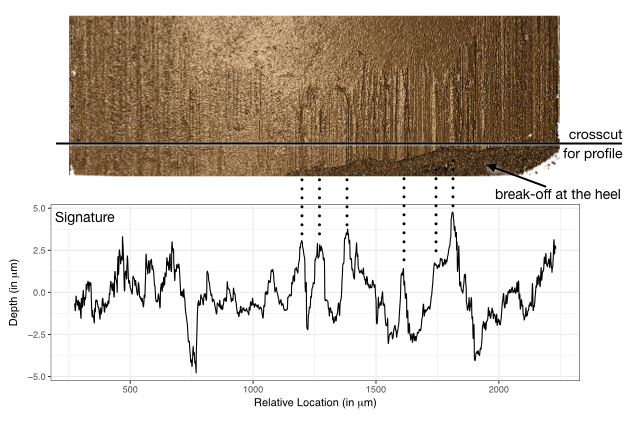
\includegraphics[width=\textwidth]{images/B6-B2-L6-rescaled.png}


\caption{\label{fig:rgl} Image of a bullet land from a confocal light microscope at 20 fold magnification (top) and a chart of the corresponding signature of the same land (bottom). The dotted lines connect some peaks visible in both visualizations.}

\end{figure}

\subsection{The Chumbley Score Test}\label{the-chumbley-score-test}

The Chumbley score algorithm takes input as two vectorized processes.
Here the processes are of the form \(z(t)\) which is a spatial process
for some location indexed with \(t\). This means that while \(z(t)\)
represents any striae, \(z(t_1)\) is a realization of the spatial
process. \(t\) here denotes a vector of equally spaced pixel locations
for the striation marks under consideration. The word `pixel' refers to
the resolution of the confocal light microscope. In the case for bullet
signatures extracted from NIST ballistics database \citep{nist} of the
Hamby study, a pixel corresponds to approximately 1.56 microns. The
vectorized processes representing two sets of striaes are therefore
shown as \(x(t_1)\), \(t_1 = 1,2,...T_1\) and \(y(t_2)\),
\(t_2 = 1,2...T_2\). Here \(x\) and \(y\) denote two instances of the
process \(z(*)\) which means two striation marks, while the indexing
\(t\) or pixel range is shown as \(t_1\) and \(t_2\) for \(x\) and \(y\)
respectively. This representation of \(t\) as \(t_1\) and \(t_2\) lets
us identify them as either of same or different lengths. The striation
marks under consideration are potentially from two different bullets
whose source needs to be identified as being same or different. \(T_1\)
and \(T_2\), as represented above, are the final pixel indexes of each
marking and therefore give the respective lengths of the markings. The
similarity in the two markings is then judged by the algorithm on the
basis of cross-correlation of a fixed and constant number consecutive
pixels (say \(k\)) taken from the two markings. This can for example be
\(k\) taken from the two indexed marking \(x(t_1)\) and \(y(t_2)\) such
that in theory \(k\) remains smaller than length of the two striae or
marks. Depending on what stage of the algorithm we are in, matching of
different pixel lengths and locations is done. This in the end,
effectively compares all possible windows that would guarantee in
quantifying the two marks or striae as coming from the same source or
not.

The algorithm works in two phases, namely, an optimization step and a
validation step, at the end of which a Mann Whitney U statistic is
calculated as a measure to differentiate between matches and
non-matches. A pre-processing step to the algorithm is to choose a
coarseness value which is used as a parameter to the lowess smoothing
function. The coarseness essentially gives the proportion of points
which influence the smooth at each value, which means larger values lead
to more smoothness. The lowess smoothing is applied to each of two sets
of vectorized striae or marks \(x(t_1)\) and \(y(t_2)\), before
proceeding to the algorithm. The algorithm starts with the optimization
step where the area of best agreement in the two markings being compared
is identified. Comparison window size is predefined. Each window of the
first marking is compared with all windows of the second marking. A
maximum correlation statistic is used to identify the region of best
agreement, with the maximum usually seen being near 1 for both cases
which is what is intuitively expected for matches, and not expected
intuitively for non matches. \citet{hadler} in their paper proposed an
improvement to this algorithm by trying to remove mutual dependence of
parameters. The mututal dependence was due to the serial correlation in
surface depth values of a marking. Also a random sampling sub step in
the validation phase makes a group of pixels to be chosen more than once
and hence introduces lack of independence in certain steps. The reason
for removing the mutual dependence was the Mann-Whitney U statistic
works under the assumption of independence of parameters. The validation
step builds on this with two sub-steps namely, same shift and different
shift. As the aim is to come up with a non-parameteric U statistic,
\citet{hadler} proposed a normalization procedure in the validation step
which goes to some extent to address the issue of mutual dependence. A
series of windows are chosen in both the same and different shift
sub-steps for the purpose of comparison. Both substeps were modified by
\citet{hadler} who introduced a deterministic rule for sampling of
windows in the same-shift and different shift as opposed to the
originally proposed random sampling by \citet{chumbley}. In th same
shift substep the chosen series of windows are at a common distance
(rigid-shifts) from the window earlier identified as the region of best
agreement in the optimization step. The correlation of these windows
generally turn out to be lower than the maximum correlation window. The
significance is that these same shift windows still have large enough
correlation values for the two markings being compared that are in
reality a match. Any choice of maximum correlation windows (where
correlation values are often near 1) for non-matches in the optimization
step are also validated by this sub-step. This is because the same-shift
correlations would not be anywhere as large for same-shift windows when
all windows in the sub-step are compared. The different shift substep on
the other hand gives perspective to the correlation values of the same
shift window correlation values. There are no rigid-shifts but different
shifts where distance from the maximum correlation window are chosen
randomly by \citet{chumbley} and deterministically as per
\citet{hadler}. This means that there is an equal possibilty of
comparing a trace segment from one marking to any trace segment or
window in the second marking.

Neither of above sets of correlation in the two sub-steps are allowed to
include the maximum correlation window as identified earlier. Therefore
the assumption is that if two markings match each other, the same-shift
correlations would be larger than the different-shift windows. And if
they are not a match the correlations in the two sets will be very
similar. The U-statistic tests for the null hypothesis that the two
markings are not a match and are therefore not made by the same source.
As given by \citet{hadler}, it is computed from the joint rank of all
correlations of both the same and different shift samples.

\begin{figure}

{\centering 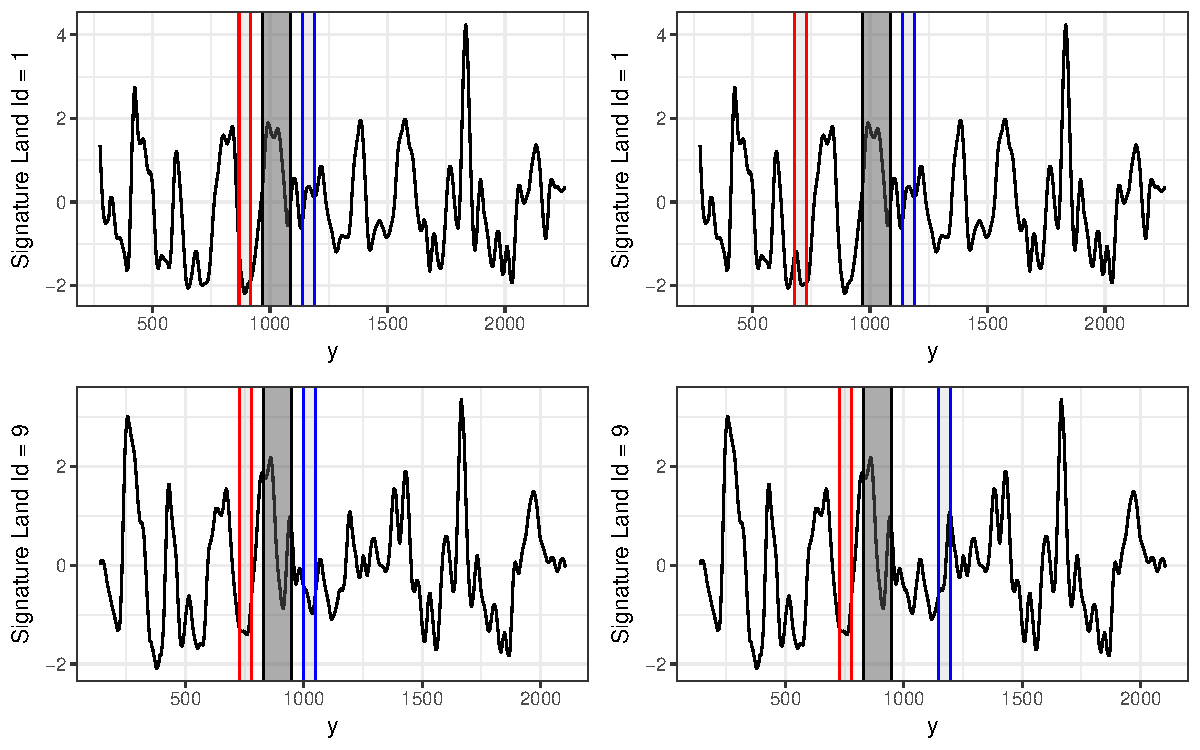
\includegraphics[width=\textwidth]{figures/win-comparison-1} 

}

\caption{ The two plots on the left show how the same shift behaves in case of a matching pair and the two plots on the right show how the different shift behaves in case of a matching pair.}\label{fig:win-comparison}
\end{figure}

\section{Simulation setup}\label{simulation-setup}

Following on similar lines to the setup of toolmarks, the first step
here is to first identify what difference does different window sizes of
optimization and the validation step have, when adapting the toolmark
method to bullets.

The marking made on bullets are smaller than toolmarks and is also less
wider. The idea is to find out possible areas of error while adapting
the score based method proposed for toolmarks, using cross-validation
setup to identify appropriate parameter settings for (a) signatures and
(b) profiles directly

\subsubsection{Signatures}\label{signatures}

Signatures of lands for all Hamby-44 and Hamby-252 scans made available
through the NIST ballistics database \citep{nist} were considered. Both
of these sets of scans are part of the larger Hamby study \citep{hamby}
and each consist of twenty known bullets (two each from ten
consecutively rifled Ruger P85 barrels) and fifteen questioned bullets
(each matching one of the ten barrels). Ground truth for both of these
Hamby sets is known and was used to assess correctness of the tests
results.

Bullet signatures being compared at this time are therefore from the
Hamby 44 and Hamby 252 data. The database setup and pre-processing
system used for choosing the Bullet signatures are as described by
\citet{aoas}. In order to choose the bullet signatures we first filter
out Land\_id for Profiles from the Hamby 44 and Hamby 252 data and
remove all NA values. Then run\_id = 3 is chosen as the signatures
generated from this run\_id give the closest match. Different run\_id's
have some different settings for generating the signatures.(The level of
smoothing does not seem to be one of them)

The bullet signatures when generated by this process already includes a
loess smoothing. Therefore, the coarseness factor is set to 1 while
running the chumbley non random algorithm for comparing different
optimization windows.The algorithm generates the same\_shift,
different\_shift, U-Stat and P\_value parameters which are then used to
calculate the errors associated with different sets of window sizes.

\subsubsection{Profiles}\label{profiles}

The profiles are cross-sectional values of the the bullet striation mark
which are chosen at an optimum height (x as used by \citet{aoas}). This
x or height is not a randomly chosen level. The rationale behind the
choice has been explained by \citet{aoas}. A region is first chosen
where the cross-correlation seems to change very less and in this region
an optimum height is chosen. The profiles generally resemble a curve
which is more or less similar to a quadratic curve (a quadratic fit to
the raw data values of the profile is not an exact fit but it does show
a similar trend). Profiles are the set of raw values representing the
striation marks, and signatures are generated from these by removal of
the inherent curvature and applying some smoothing (the signatures
generated by \citet{aoas} use a loess function for smoothing).

Similar to signatures the run\_id = 3 was used when applying the
chumbley algorithm using the database setup given by \citet{aoas} of
Hamby-44 and Hamby-252 datasets, on the profiles. The run\_id not only
defines the level of smoothing but also signifies the chosen height at
which the profiles were selected initially. Another important aspect is
the range of horizontal values (which is referred to as the y values in
\citet{aoas}) in the signatures. These have already been pre-processed
in the database to not include any grooves.

Therefore for the sake of comparison the run\_id = 3 is still chosen so
as to ensure that the horizontal values remain the same as that of the
signatures. This also gives us profiles with the grooves removed.

The idea therefore is to first use these raw values of the profile
directly in the chumbley algorithm, and see how the algorithm performs
for different coarseness values (smoothing parameter as referred in the
function lowess used in the chumbley algorithm).

\pagebreak

\section{Results}\label{results}

We used the adjusted Chumbley method as proposed in \citet{hadler} and
implemented in the R package \texttt{toolmaRk} \citep{toolmark} on all
pairwise land-to-land comparisons of the Hamby scans (a total of 85,491
comparisons) with the pairwise sets for the comparisons given in the
table \ref{tab:param}.

\begin{table}[!h][!h]
\caption{\label{tab:param}Overview of parameter settings used for optimization and validation windows for bullet land signatures.}

\centering
\resizebox{\linewidth}{!}{\resizebox{\linewidth}{!}{\begin{tabular}[t]{lrrrrrrrrrrrrrrrrrr}
\toprule
wo & 50 & 50 & 60 & 60 & 80 & 80 & 90 & 90 & 100 & 100 & 110 & 110 & 120 & 120 & 120 & 120 & 120 & 130\\
wv & 30 & 50 & 30 & 50 & 30 & 50 & 30 & 50 & 30 & 50 & 30 & 50 & 10 & 20 & 30 & 50 & 60 & 30\\
\bottomrule
\end{tabular}}}
\centering
\begin{tabular}[t]{lrrrrrrrrrrrrrrr}
\toprule
wo & 130 & 140 & 140 & 150 & 150 & 160 & 160 & 200 & 200 & 200 & 240 & 240 & 280 & 280 & 320\\
wv & 50 & 30 & 50 & 30 & 50 & 30 & 50 & 20 & 30 & 50 & 30 & 50 & 30 & 50 & 30\\
\bottomrule
\end{tabular}
\end{table}

\begin{table}[!h]
\caption{\label{tab:confusion}Confusion Table for different optimization window sizes with validation window size as 30.}

\centering
\begin{tabular}[t]{llrl}
\toprule
\hspace{1em}\hspace{1em}signif & match & Freq & Type\\
\midrule
\addlinespace[0.5em]
\multicolumn{4}{l}{\textbf{Size of Optimization Window = 280}}\\
\hspace{1em}FALSE & FALSE & 78909 & True Negative\\
\hspace{1em}TRUE & FALSE & 4192 & False Positive (Type I)\\
\hspace{1em}FALSE & TRUE & 446 & False Negative (Type II)\\
\hspace{1em}TRUE & TRUE & 731 & True Positive\\
\bottomrule
\end{tabular}
\centering
\begin{tabular}[t]{llrl}
\toprule
signif & match & Freq & Type\\
\midrule
\addlinespace[0.5em]
\multicolumn{4}{l}{\textbf{Size of Optimization Window = 120}}\\
\hspace{1em}FALSE & FALSE & 79249 & True Negative\\
\hspace{1em}TRUE & FALSE & 4523 & False Positive (Type I)\\
\hspace{1em}FALSE & TRUE & 386 & False Negative (Type II)\\
\hspace{1em}TRUE & TRUE & 854 & True Positive\\
\bottomrule
\end{tabular}
\centering
\begin{tabular}[t]{llrl}
\toprule
signif & match & Freq & Type\\
\midrule
\addlinespace[0.5em]
\multicolumn{4}{l}{\textbf{Size of Optimization Window = 80}}\\
\hspace{1em}FALSE & FALSE & 79477 & True Negative\\
\hspace{1em}TRUE & FALSE & 4503 & False Positive (Type I)\\
\hspace{1em}FALSE & TRUE & 463 & False Negative (Type II)\\
\hspace{1em}TRUE & TRUE & 781 & True Positive\\
\bottomrule
\end{tabular}
\end{table}

\subsection{Signatures}\label{signatures-1}

Figure \ref{fig:type2} gives an overview of type II error rates observed
when varying the window size in the optimization step. Two levels of
validation window size 30 and 50 were chosen as to compare the error
rates for different nominal type I errors. We notice that the trends for
these nominal type I errors are similar and in most cases a validation
window of 50 has higher type II error than for 30. A change in this
trend is seen for a 0.05 \(\alpha\) level, although the difference
between the two windows is very small for this case. We can also notice
an obvious trend of increase in the Type II error as the window of
optimization increases and see a minimum around the optimization window
size of 120 pixels. Hence we are inclined to choose a smaller validation
window size and optimization window as 120.

Table \ref{tab:confusion} shows the confusion tables with the
classification of type I and type II errors and how the numbers change
with a change in the optimization window. The windows represent areas to
the left of the window with minimum type II, near the minimum type II
window and to the far right of the minimum type II error

\begin{figure}

{\centering 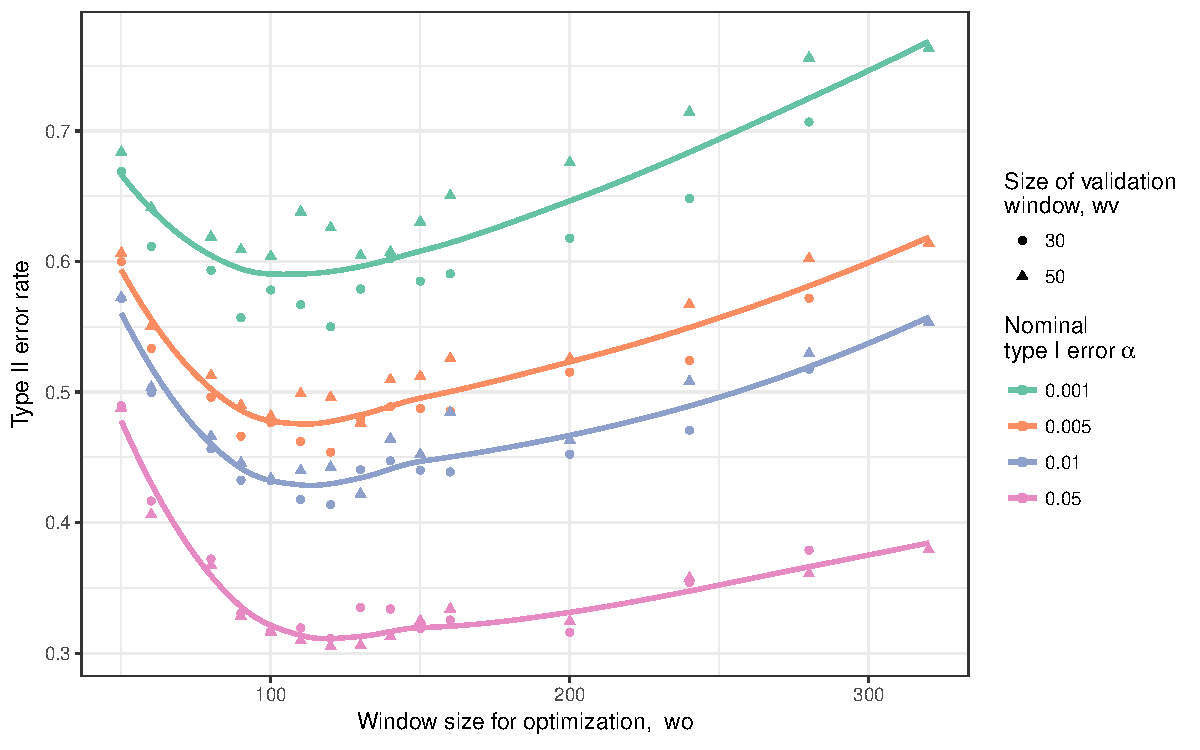
\includegraphics[width=\textwidth]{figures/type2-1} 

}

\caption{Type II error rates observed across a range of window sizes for optimization $wo$. For a window size of $wo = 120$ we see a drop in type II error rate across all type I rates considered. Smaller validation sizes $wv$ are typically associated with a smaller type II error.}\label{fig:type2}
\end{figure}

Figure \ref{fig:type1} compares nominal (fixed) type I error and
actually observed type I errors for the parameter settings in table
\ref{tab:param}. With an increasing size of the window used in the
optimization step the observed type I error rate decreases (slighty).
This means as the optimization window increase the observed type I error
rate gets smaller. A smaller validation window on the other hand, tends
to be associated with a higher type I error rate. This can be better
imagined for a given window of optimization, where the actual Type I
error is comparable to the nominal level for only a select few
validation window sizes. For these comparable validation window sizes of
30 and 50 as done here, the actual type I error increases very slightly
and can be seen in Figure \ref{fig:type1}. This increase is not as much
when compared to the variation seen with the optimization window sizes.
This effect might be related to the increasing number of tests that fail
for larger optimization window sizes, in particular for non-matching
striae (see fig \ref{fig:missings}).

\begin{figure}

{\centering \includegraphics[width=\textwidth]{figures/type1-1} 

}

\caption{Comparison of observed and nominal type I error rates  across a range of window sizes for optimization $wo$. The horizontal line in each facet indicates the nominal type I error rate.}\label{fig:type1}
\end{figure}

\begin{figure}

{\centering 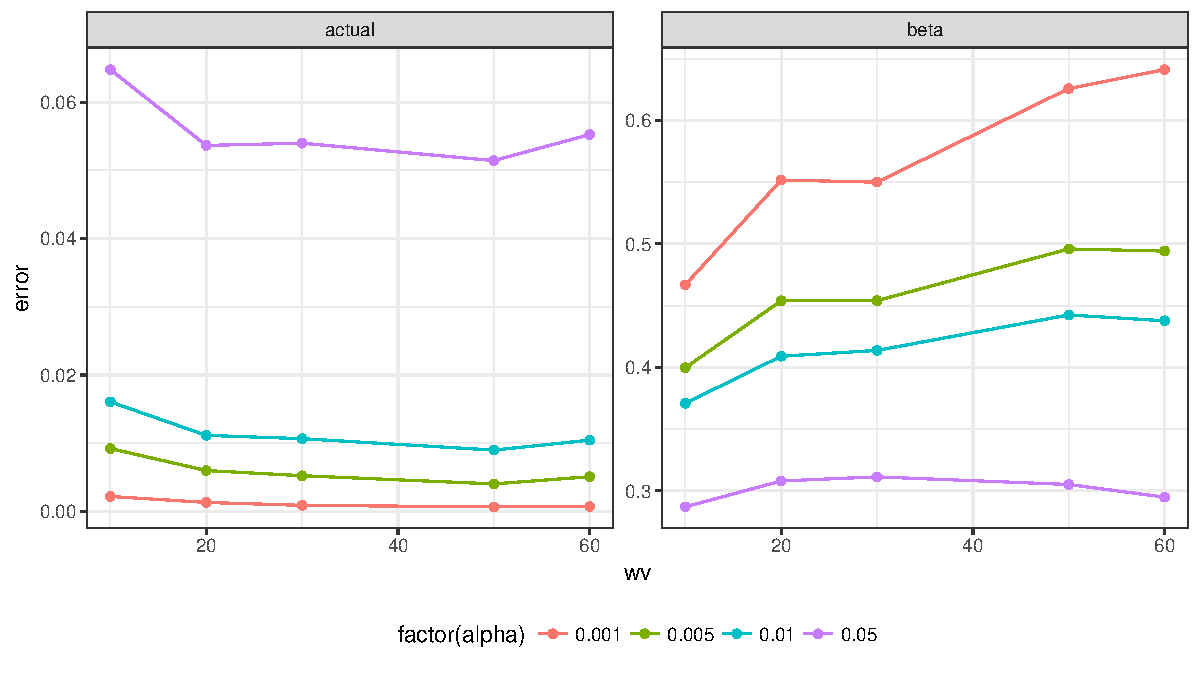
\includegraphics[width=\textwidth]{figures/wo120-1} 

}

\caption{The figure on the left shows the actual Type I error while the figure on the right shows the Type II error for different validation window sizes and different chosen nominal alpha levels when the size of the optimization window = 120}\label{fig:wo120}
\end{figure}

The actual type I error and type II error for signatures were also
compared for different validation window sizes. Figure \ref{fig:wo120}
shows the actual rates for different nominal \(\alpha\) levels. We can
see that the type II error rises with higher validation windows for the
smaller nominal \(\alpha\) levels while for the nominal \(\alpha\) =
0.05 its almost constant.

\begin{figure}

{\centering 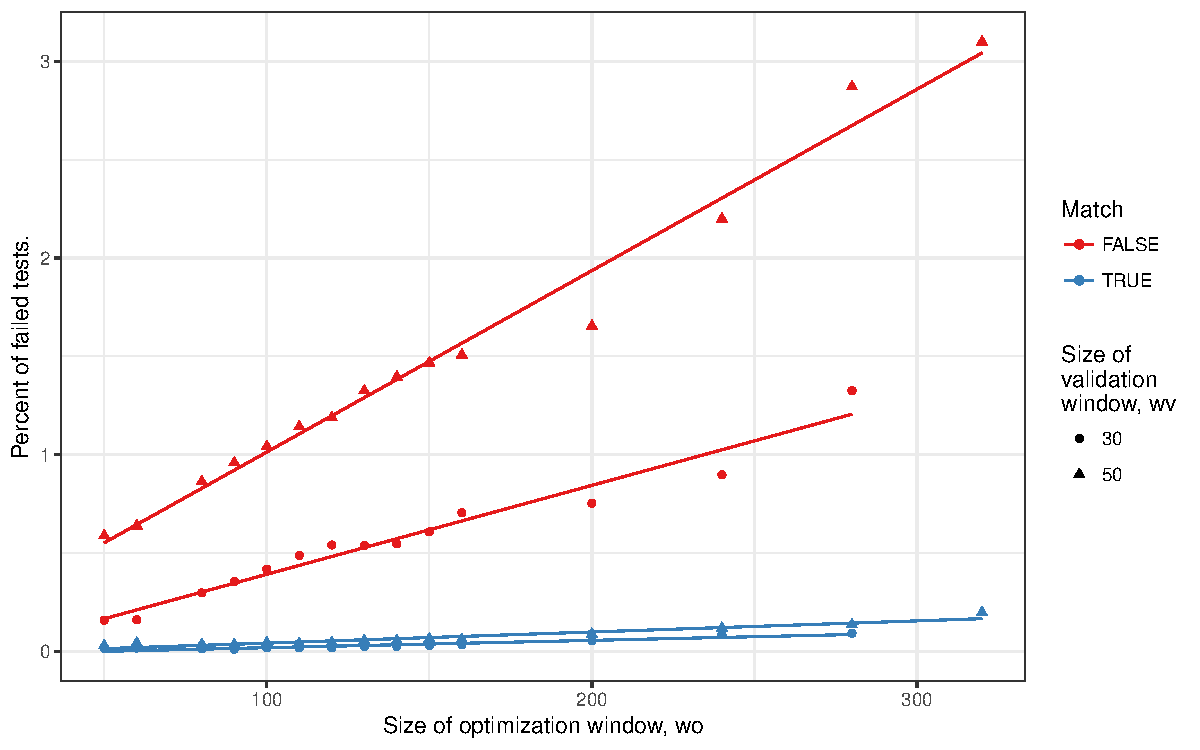
\includegraphics[width=\textwidth]{figures/missings-1} 

}

\caption{Number of failed tests by the window optimization size, wo, and ground truth.}\label{fig:missings}
\end{figure}

\begin{table}

\caption{\label{tab:lms}Estimates of the increase in percent of failed tests corresponding to a 100 point increase in the optimization window.}
\centering
\begin{tabular}[t]{lrrr}
\toprule
match & wv & estimate & std.error\\
\midrule
FALSE & 30 & 0.503 & 0.028\\
FALSE & 50 & 0.922 & 0.035\\
TRUE & 30 & 0.043 & 0.004\\
TRUE & 50 & 0.056 & 0.005\\
\bottomrule
\end{tabular}
\end{table}

Figure \ref{fig:missings} gives an overview of the number of failed
tests, i.e.~tests in which a particular parameter setting did not return
a valid result. This happens, when the shift to align two signatures is
so large, that the remaining overlap is too small to accommodate windows
for validation. The problem is therefore exacerbated by a larger
validation window. Figure \ref{fig:missings} also shows that the number
of failed tests is approximately linear in the size of the optimization
window. Test results from different sources have a much higher chance to
fail, raising the question, whether failed tests should be treated as
rejections of the null hypothesis of same source. For known non-matches
there is a higher possibility that in the optimization pair of windows
where cross-correlations are maximum are too far apart, and same shifts
of this order hit the end of the signature.

\subsection{Profiles}\label{profiles-1}

Figure \ref{fig:prof_missings} (a) shows the type II error rates for
profiles for the optimization window 120 and validation window 30 with
varying level of coarseness. We can see that the type II error for all
the nominal \(\alpha\) levels is lowest in the range of 0.20 to 0.35.
Therefore, a value of 0.25 can be used keeping in mind it keeps the type
II error lowest while runnning simulations. Thus for comparisons of
different window sizes etc as seen in the differnt parts of Figure
\ref{fig:prof_missings} this coarseness value is used.

On the other hand Figure \ref{fig:prof_missings} (b) shows if the
coarseness level set in the chumbley agorithm has any effect on the
signatures, which are pre-processed and already smoothed to a certain
extent. From Figure \ref{fig:prof_missings} (b) we can notice that for
different nominal \(\alpha\) levels, the type II error fluctuates
slightly but does not change much, thereby helping us conclude that the
coarseness levels set in the LOWESS smoothing in the chumbley alggorithm
does effect the type II error much for signatures.

\subsubsection{Comparison of profiles and
signatures}\label{comparison-of-profiles-and-signatures}

Another reason for failed tests can be incorrect identification of
maximum correlation windows in the optimization step as seen in figure
\ref{fig:prof_missings}(d) because of the level of smoothing, as too
much smoothing would subdue intricate features that might otherwise help
in the correlation calculations and correct identification of maximum
correlation windows irrespective of the size. This would again cause a
simiar effect as explained for figure \ref{fig:missings} with validation
windows, irrespective of size, during the shifts end up at the ends of
the markings resulting in an invalid calculation and failed comparison
attempt.

In figure \ref{fig:prof_missings}(d) and (f), we compare profiles and
signatures on the basis of number of failed tests. The profiles chosen
for figure \ref{fig:prof_missings}(f) have a constant coarseness of 0.25
and window of optimization as 120. The signatures in this case are not
smoothed using the chumbley algorithm step of LOWESS smoothing. Instead
signatures are used as calculated by \citet{aoas}. The smoothing in
these signatures were determined and fixed on the basis of their
performance in the random forest based algorithm proposed by
\citet{aoas}. The comparison of profiles and signatures with variation
of validation window size therefore is made on even footing. The trends
are similar to figure \ref{fig:missings} in the sense that for known
non-matches the number of failed tests are more for both signatures and
profiles and increasing linearly with the validation window size. The
problem is however, worse for profiles which has higher number of failed
tests than signatures for all validation windows.

The total error for different validation window sizes for signatures and
profiles can be seen in figure \ref{fig:prof_missings} (e).The
optimization window size is 120 and profiles are calculated at a default
0.25 coarseness level while signatures as before are not smoothed again
in the modified chumbley algorithm. We can see that the total error is
always higher for profiles as compared to signatures for all sizes of
validation window.

\begin{figure}

{\centering \includegraphics[width=\textwidth]{figures/prof_missings-1} 

}

\caption{Row 3:  Total error and Number of failed tests by the window validation size, wv, and ground truth, Row 2: Total error and Number of failed tests with Coarseness for both profiles and signatures, Row 1: Type II error for different coarseness levels as used in the modified chumbley algorithm for profiles and signatures}\label{fig:prof_missings}
\end{figure}

\pagebreak

\subsection{Conclusion}\label{conclusion}

The results suggest that the Nominal type I error \(\alpha\) value shows
dependence on the size of the window of optimization. For a given window
of optimization the actual Type I error is comparable to the nominal
level for only a select few validation window sizes and for comparable
validation window sizes of 30 and 50 as done here, the actual type I
error does not seem to vary as much as it varies with the optimization
window sizes . A Test Fail, i.e.~tests in which a particular parameter
setting did not return a valid result, happens, when the shift to align
two signatures is so large, that the remaining overlap is too small to
accommodate windows for validation, depends on whether known-match or
known non-matches has predictive value, with test results from different
sources having a much higher chance to fail. On conducting an analysis
of all known bullet lands using the adjusted chumbley algorithm, Type II
error was identified to be least bad for window of validation 30 and
window of optimization 120. In case of unsmoothed raw marks (profiles),
Type II error increases with the amount of smoothing and least for
LOWESS smoothing coarseness value about 0.25 or 0.3. In an effort to
identify the level of adaptiveness of the algorithm, comparisons were
made between signatures and profiles. Their comparison with respect to
validation window size for a fixed optimization window size suggested
that, profiles have a total error (i.e all incorrect classification of
known-matches and known non-matches) greater than or equal to the total
error of signatures for all sizes of validation window. Profiles also
fail more number of times than signatures in a test fail (for different
coarseness keeping windows fixed and also for different validation
windows keeping coarseness fixed) which lets us conclude that the
behaviour of the algorithm for the profiles instead of pre-processed
signatures is not better. Finally it should be noted that the current
version of the adjusted chumbley algorithm seems to fall short when
compared to other machine-learning based methods \citet{aoas}, and some
level of modification to the deterministic algorithm needs to be
identified and tested that would reduce the number of incorrect
classifications.

\bibliographystyle{agsm}
\bibliography{bibliography}

\end{document}
